\documentclass[10pt,a4paper,notitlepage]{report}
\usepackage[utf8]{inputenc}
\usepackage{amsmath}
\usepackage{amsfonts}
\usepackage{amssymb}
\usepackage{hyperref}
\usepackage[margin=1in]{geometry}
\usepackage{fancyhdr}
\usepackage[svgnames]{xcolor}
\usepackage{graphicx}
\usepackage{minted}

\usemintedstyle{manni}
\pagestyle{fancy}
\fancyhead[L]{\small Decoding Neuronal EEG Activity}
\fancyhead[R]{\small\textsc{Problem 3}}
\renewcommand{\headrulewidth}{0.4pt}
\fancyfoot[C]{\thepage}

%\newcommand{\code}[1]{\colorbox{lightgray}{\texttt{#1}}}

\begin{document}

\paragraph*{GENERAL REMARKS} The programming problems require you to fill the gaps in the provided MATLAB scripts. Use the problem description below and the comments in the code to solve the problems. The missing parts are typically indicated by '\texttt{...}' (not to be confused with line breaks!), where each '\texttt{...}' might be replaced by multiple lines of code. Following the provided code is recommended but only leads you to one of many possible solutions. If some part of the code seems unclear or counterintuitive to you, feel free to depart from it. Be aware, however, that the suggested variable names and structures are typically used later in the script, e.g. for plotting, and occur again in other scripts and problems. In any case, your code should produce the same output as the Musterlösung. \textbf{Note}: To be able to run the code, you must have the Statistics, Signal Processing, Image Processing, and Wavelet toolboxes installed, and you must have the folder \texttt{utility} and all subfolders as well as the location of the ECG/EEG datasets added to your MATLAB path.

\section*{Problem 3}
In this problem, we will analyze and classify human EEG data, analogous to Scheller et al., 2009. Have a look at the paper to get an overview, but be aware that data and processing are not identical to our problem. The data were recorded from one subject under three different levels of anesthesia while constantly presenting short auditory stimuli. Analogous to the ECG data from problem 2, we will eventually try to discriminate data from two arbitrary blocks. However, here we will perform multiresolution analysis (MRA) in order to compute features from the wavelet-transformed signal. The scripts \texttt{runEEG<1,2,3>.m} will successively build the final program, and we will make further adjustments to the classification function, yielding \texttt{modelFitVal3.m}.

\section*{Part 1: Preprocessing, Understanding MRA}
In \texttt{runEEG1.m} we will first examine the data from block 1, corresponding to normal wakefulness. The data are already epoched, yielding the 3 dimensions \textit{channels}, \textit{sample points}, and \textit{epochs}. Each epoch contains 3 consecutive sweeps, i.e. post-stimulus signal sequences, of approx. 102 ms each. Eventually, we will be interested in the middle sweep only.

We begin by specifying the sampling frequency of 5 kHz, loading the signal, and extracting dimensions. Then we plot the first 3 epochs for all channels of the raw signal in a qualitative way.

\begin{minted}[xleftmargin=1cm]{matlab}
srate = 5000;
load('block1')
[nChans, nPts, nEpochs] = size(EEG.data);

data3 = reshape(EEG.data(:, :, 1:3), nChans, 3*nPts);

...

pause
\end{minted}

There is nothing to edit so far. The plot will give you a general picture of the signal in each channel. After plotting, the code awaits a key press to continue. You may want to run these first lines of code right now. (E.g. mark the respective lines and press F9).

Next, we initialize further figures, load a high-pass and low-pass filter, and start iterating over channels.

\begin{minted}[xleftmargin=1cm]{matlab}
f1 = figure('Name', 'WT scales, epoch 1, Ch 1', ...
    'units', 'normalized', 'outerposition', [0 0 0.5 1]);
f2 = figure('Name', 'reconstructed ERP, Ch 1', ...
    'units', 'normalized', 'outerposition', [0.5 0 0.5 1]);

load('filterLP_1000_1200.mat')
load('filterHP_0.1_10.mat')

for iChan=1:nChans
\end{minted}

As in problem 2, use \texttt{fdatool} to construct a high-pass filter with transition band edges at 0.1 Hz and 10 Hz and a low-pass filter with transition band edges at 1000 Hz and 1200 Hz. Store the filter coefficients as \texttt{filterHP} and \texttt{filterLP} under the given file names. Note that filters must not exceed a certain length for the \texttt{filtfilt} function to work. Find a tradeoff between filter length and precision of the frequency repsonse.

Now, for each channel, we extract the epoched signal and get rid of the first singleton dimension and then filter and baseline-correct the data.

\begin{minted}[xleftmargin=1cm]{matlab}
signal = squeeze(EEG.data(iChan, :, :));

signal = filtfilt(filterHP, 1, signal);
signal = filtfilt(filterLP, 1, signal);
signal = cleanAC(signal, 50, srate);
baseline = ...
signal = signal - ...
\end{minted}

We only keep the band-pass filtered signal, and, in addition, apply a 50 Hz notch filter using \texttt{cleanAC}. Implement robust baseline correction by subtracting from each epoch the mean signal around the time of the 2nd sweep onset. Use a window of roughly 100 points. Note that, unlike in problem 2, the data is already 2-dimensional. The \texttt{repmat} function or a for-loop should do the trick.

Next, we compute the event-related potential (ERP) for the middle sweep, i.e. we average the middle 512 points of the signal over all epochs. \texttt{ERP} should be a vector of length 512.

\begin{minted}[xleftmargin=1cm]{matlab}
ERP = ...
\end{minted}

The next line of code computes the wavelet transform. It calls the function \texttt{MRA\_stationary\_fast} using a Daubechies 4 wavelet to transform the signal at 7 distinct frequency bands, or scales of resolution, centered around approx. 14 Hz, 28 Hz, 56 Hz, 112 Hz, 223 Hz, 446 Hz, and 893 Hz. This is known as multiresolution analysis (MRA).

\begin{minted}[xleftmargin=1cm]{matlab}
sWT = MRA_stationary_fast(signal, 'db4', srate);
\end{minted}

The maximum number of scales is dictated by the length of the signal. The function actually computes one more scale, but we will only consider the first 7. This means we get 7 wavelet-filtered signals for each original signal. These are stored in \texttt{sWT.scales}.

To demonstrate that MRA is a (theoretically) loss-free transformation of the signal, we now reconstruct the signal by adding up the scales one by one.

\begin{minted}[xleftmargin=1cm]{matlab}
WT2ERP = nan(512, 7);
for iScale=1:7
    tmp = sum(...);
    WT2ERP(:, iScale) = mean(...);
end
\end{minted}

\texttt{WT2ERP} should contain in the $i$th column the sum of scales $1$ to $i$ for the middle sweep, averaged over all epochs.

Part 1 is finished. \texttt{runEEG1.m} should produce an overview of all raw channels for the first 3 epochs, followed, after a key press, by a series of figure pairs, advanced at each further key press.

\vspace{1cm}
\hspace{-1cm} 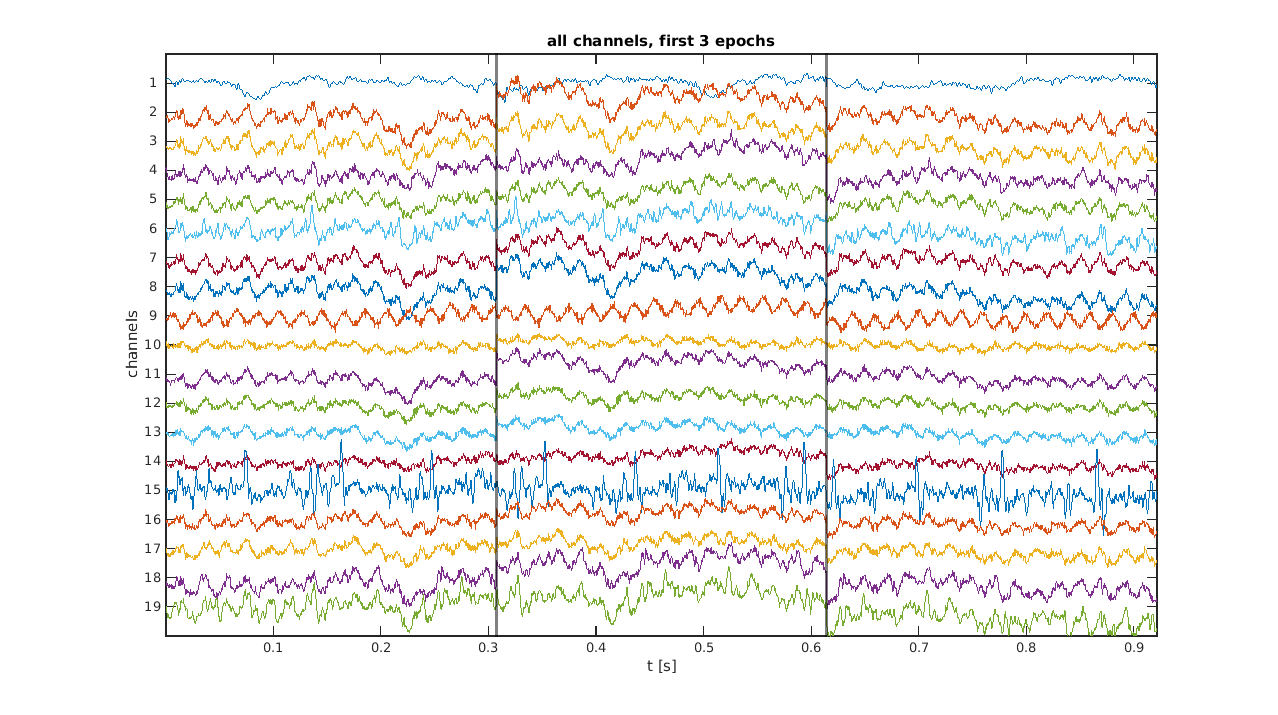
\includegraphics[scale=0.5]{p3fig1.png}

\hspace{-1cm} 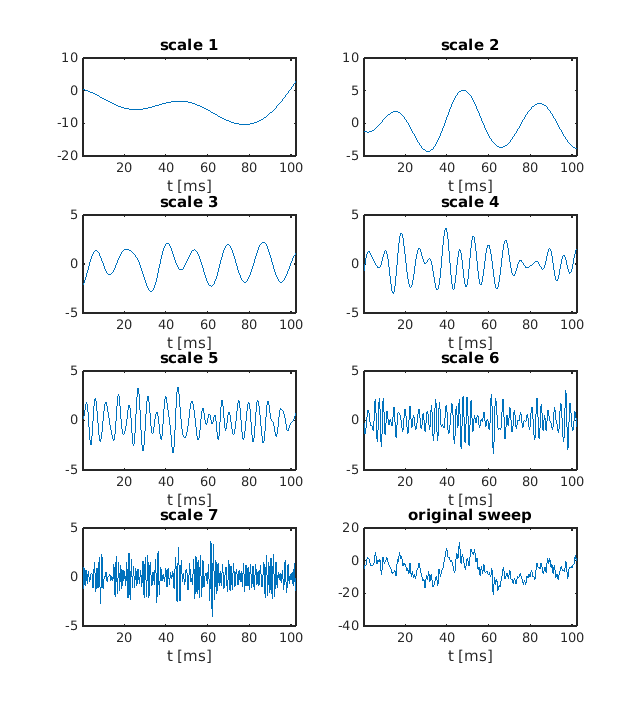
\includegraphics[scale=0.5]{p3fig2.png}
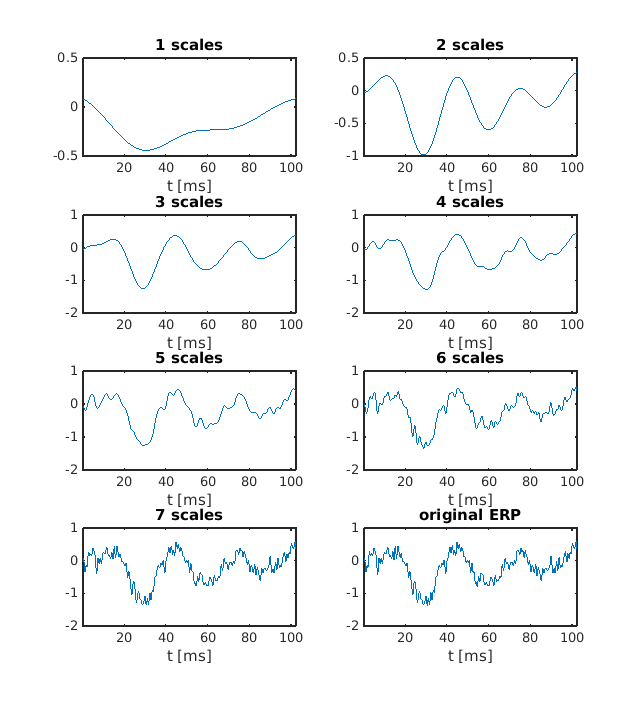
\includegraphics[scale=0.5]{p3fig3.png}
\vspace{5mm}

Each pair of figures shows the MRA decomposition of the middle sweep of the first epoch (left) and the reconstruction of the ERP (right), for the current channel (denoted in the title bars). Note how the reconstruction becomes more and more similar to the original ERP. Also, observe the differences among channels when advancing through the figures. Do some channels look faulty or overly noisy? Re-run the script for blocks 2 and 3.

\section*{Part 2: Amplitude, Phase, PLV}
In \texttt{runEEG2.m} we will process one channel from all 3 blocks and plot some relevant features. We set the sampling rate, load the filters, set a pack size for the computation of PLVs and then specify one channel to use for analysis, before iterating over blocks.

\begin{minted}[xleftmargin=1cm]{matlab}
srate = 5000;
load('filterHP_0.1_10.mat')
load('filterLP_1000_1200.mat')
packSize = 11;
useChan = ...

for B=1:3
\end{minted}

Based on your plots from part 1, choose a channel that you think is technically okay in all 3 blocks and representative of the overall signal.

For each of the 3 blocks, we now analyze the signal. We filter and baseline-correct the signal and perform MRA as before. Copying your lines from part 1 should be enough.

\begin{minted}[xleftmargin=1cm]{matlab}
load(['block', num2str(B)])
signal = squeeze(EEG.data(useChan, :, :));
[nPts, nEpochs] = size(signal);

signal = filtfilt(filterHP, 1, signal);
signal = filtfilt(filterLP, 1, signal);
signal = cleanAC(signal, 50, srate);
baseline = ...
signal = signal - ...

sWT = MRA_stationary_fast(signal, 'db4', srate);
\end{minted}

We now compute instantaneous amplitude and phase. This is very similar to the ECG problem, but the data has an additional dimension now because we use the 7-fold wavelet transform instead of the original signal. For each scale separately, instantaneous amplitude (i.e. the amplitude envelope of the signal) is computed as the absolute value of the analytic signal, and instantaneous phase is computed as its angle. Again, we unwrap the phase and correct for baseline, this time subtracting from each epoch its value right before the middle sweep onset. Amplitude will not be baseline-corrected because we're interested in absolute values along the middle sweep.

\begin{minted}[xleftmargin=1cm]{matlab}
Amp = nan(nPts, nEpochs, 7);
Phase = nan(nPts, nEpochs, 7);
for iScale=1:7
    thisScale = sWT.scales(:, :, iScale);
    Amp(:, :, iScale) = ...
    phaseTmp = unwrap(...);
    Phase(:, :, iScale) = phaseTmp - ...
end
\end{minted}

Lastly, we compute the phase locking values. Extend the code from problem 2 by the additional dimension. Again, this is a pointwise operation, so you can process each pack in one go.

\begin{minted}[xleftmargin=1cm]{matlab}
margin = floor(packSize/2);
PLV = nan(nPts, nEpochs, 7);
for iEpoch=margin+1:nEpochs-margin
    thisPack = ...
    PLV(:, iEpoch, :) = ...
end
\end{minted}

Part 2 is finished. Your code should produce 3 figures like the one below, each showing, per block, the amplitude, phase, and PLV for the 7 MRA scales. For visibility, only a few of the epochs are plotted for amplitude and phase.

\vspace{1cm}
\hspace{-1cm} 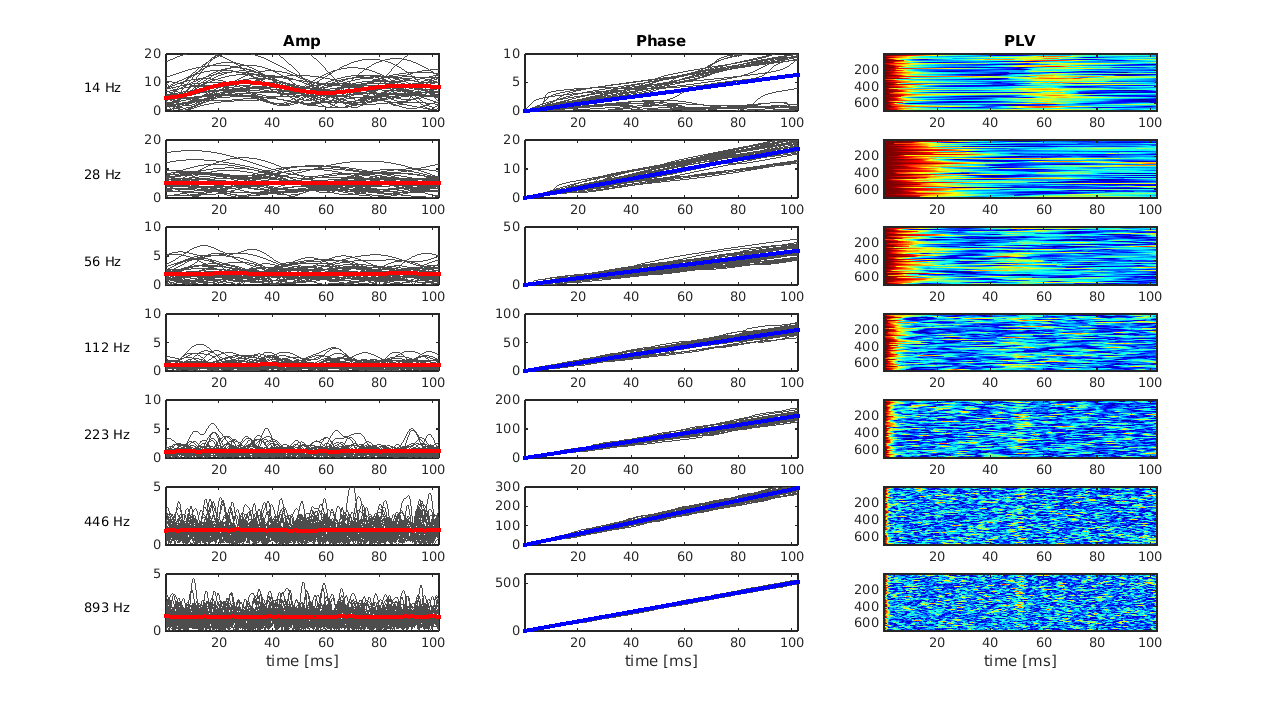
\includegraphics[scale=0.5]{p3fig4.png}
\vspace{5mm}

Compare the 3 blocks, and the scales within each block. Can you make out any differences in frequency content or phase locking strength? You can zoom in on the first 15 ms of all plots by pressing any key.


\section*{Part 3: Classification}
In part 3, we will process and classify 2 of the 3 blocks. \texttt{runEEG3.m} begins as before and also specifies the 2 blocks we want to analyze and initializes the feature structure.

\begin{minted}[xleftmargin=1cm]{matlab}
srate = 5000;
load('filterHP_0.1_10.mat')
load('filterLP_1000_1200.mat')
packSize = 11;
useBlocks = [1 3];
useChan = ...
Features = struct('Amp', [], 'PLV', []);
\end{minted}

The analysis section of the script should be almost identical to part 2. In the end, we store 2 3-dimensional matrices for each block of data, containing amplitude and PLV, respectively.

\begin{minted}[xleftmargin=1cm]{matlab}
for B=1:2

	...
	
    Features(B).Amp = Amp(:, margin+1:end-margin, :);
    Features(B).PLV = PLV(:, margin+1:end-margin, :);

end
\end{minted}

In the classification section, we first define some time points from where to sample the features. In consistence with Scheller et al., 2009, we want to examine wave V of the brainstem auditory evoked potential (BAEP), which appears during the first few milliseconds after the stimulus. Try to infer from the paper a vector of 5 sample points along wave V of the 2nd sweep.

\begin{minted}[xleftmargin=1cm]{matlab}
t = ...
\end{minted}

Next, we construct the feature matrix, analogous to problem 2. Each row will now contain 70 entries (amplitude and PLV of 7 MRA scales at 5 sample points). The order of columns doesn't matter.

\begin{minted}[xleftmargin=1cm]{matlab}
nEpochs = min(size(Features(1).Amp, 2), size(Features(2).Amp, 2));
X = nan(2*nEpochs, 70);
for B=1:2
    ...
end
\end{minted}

The remainder of the script is already complete. As before, it calls the classification function to train and cross-validate the logit, linear-kernel SVM and RBF-kernel SVM models.

\begin{minted}[xleftmargin=1cm]{matlab}
kCross = 10;
L = [ones(nEpochs, 1); zeros(nEpochs, 1)];
modelType = {'logreg', 'linsvm', 'rbfsvm'};
for iModel=1:3
    pCorrect = modelFitVal3(X, L, kCross, modelType{iModel});
    fprintf('\nPerformance %6s: %3i %%\n', modelType{iModel}, round(100*pCorrect));
end
\end{minted}

You're basically done. \texttt{runEEG3.m} should print the cross-validated performance of the 3 models. Ideally, you should see numbers above 85 \% for all 3 models, with the RBF SVM classifier performing best. In any case, try to optimize accuracy and runtime of the models. Transforming features into a new basis might be an idea. Also, have a look into \texttt{modelFitVal3.m}. So far, the function is identical to the Musterlösung from problem 2. Find out how to change the SVM parameters and optimize the classifiers. In the end, the logit model and linear SVM should perform close to 90 \%, and the RBF SVM close to 100 \%.

\end{document}
